\documentclass{standalone}
\usepackage{tikz}
\usetikzlibrary{patterns, positioning}
\usepackage[sfdefault]{ClearSans} %% option 'sfdefault' activates Clear Sans as the default text font
\usepackage[T1]{fontenc}

\begin{document}
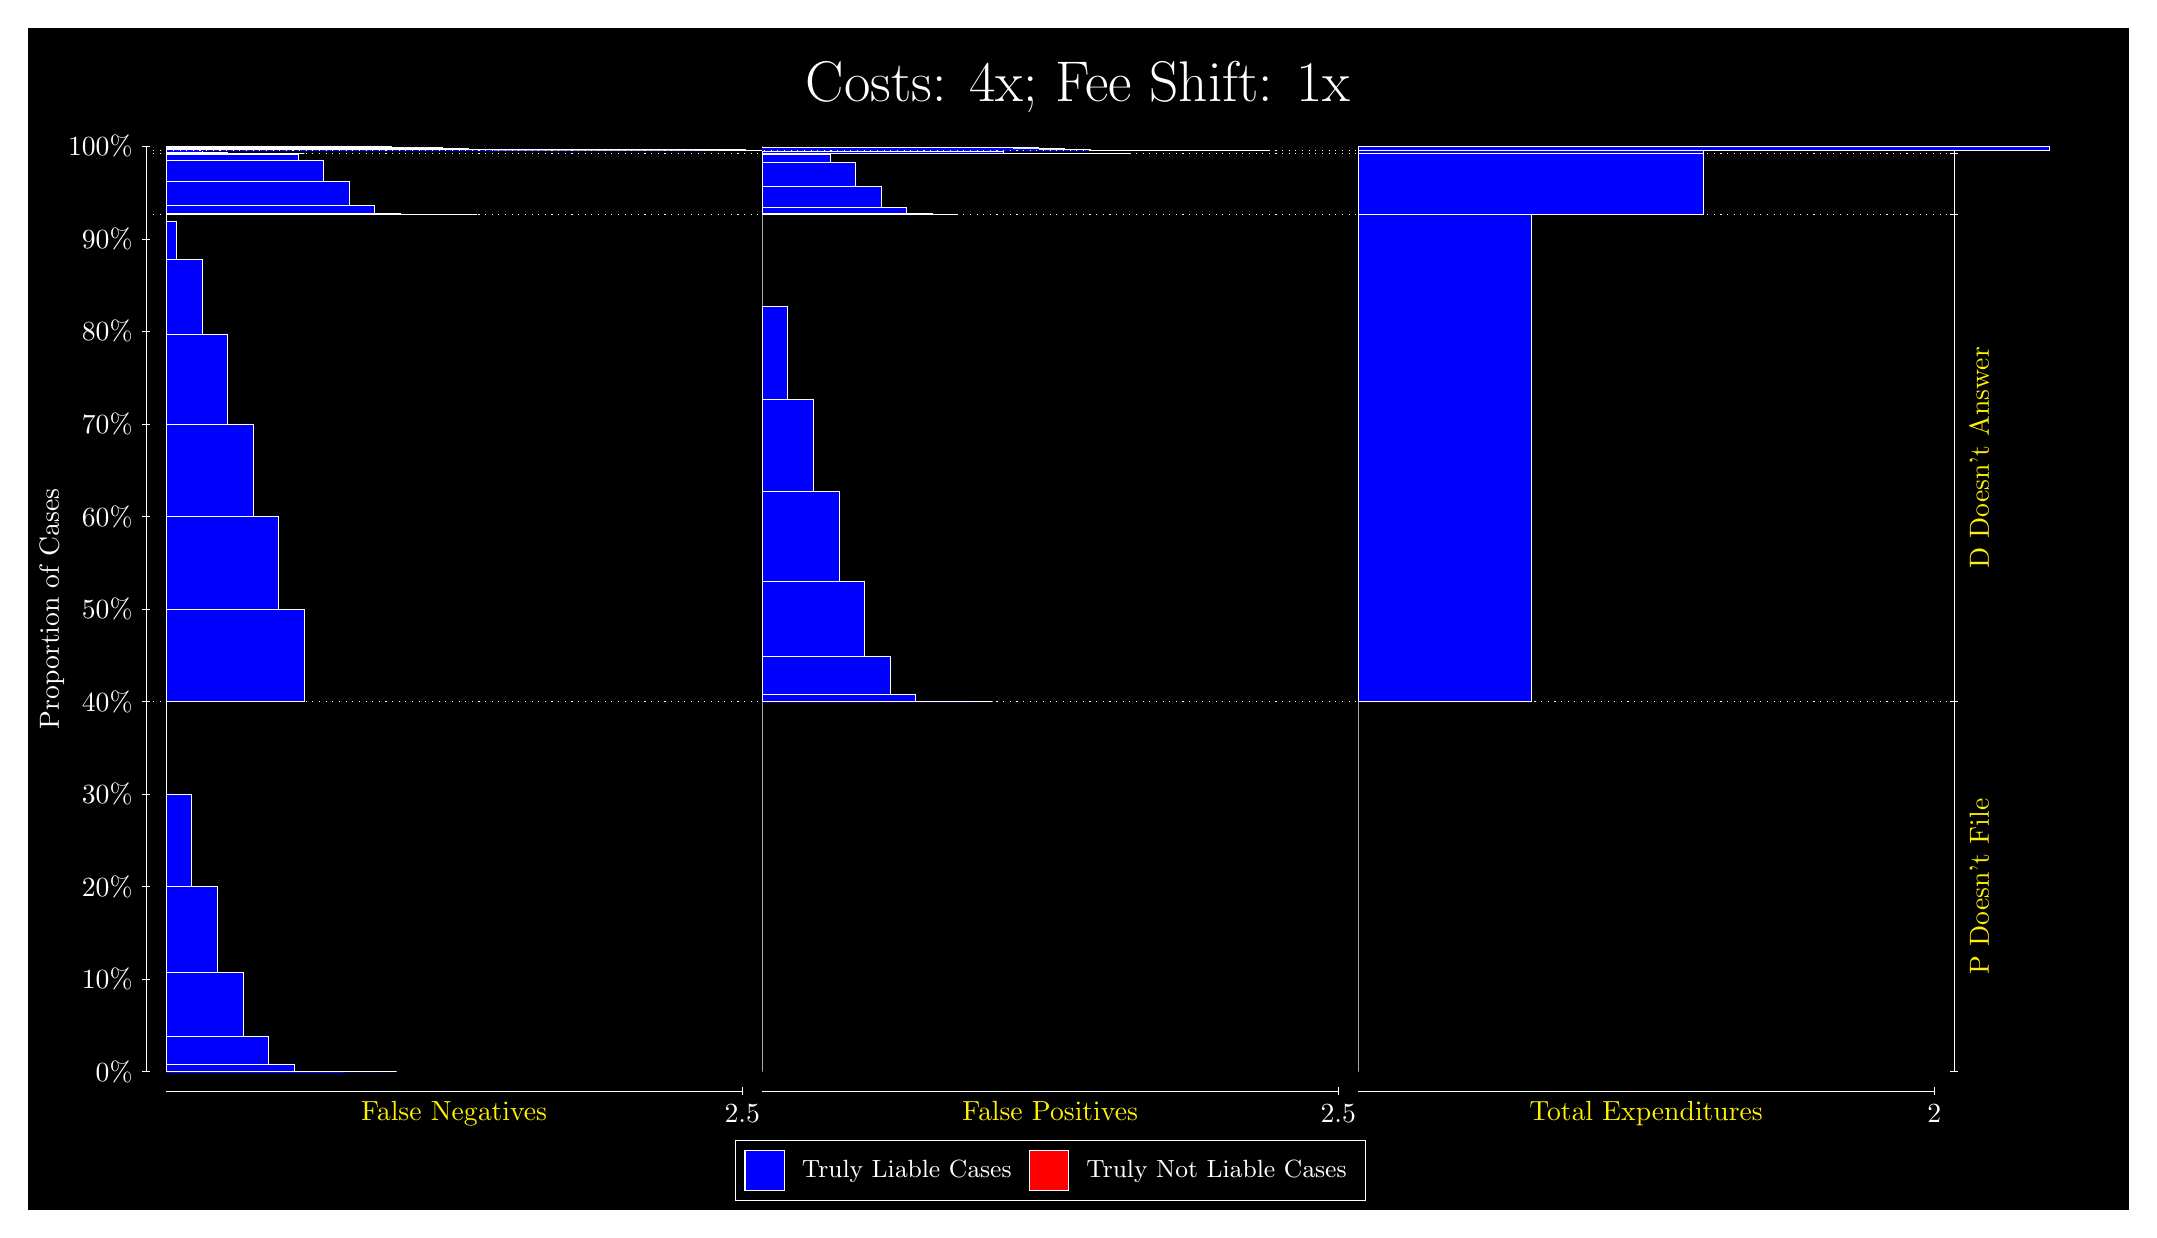
\begin{tikzpicture}
\draw[fill=black] (0,0) rectangle (26.667,15);
\draw[text=white] (0,13.5) rectangle (26.667,15) node[midway] {\huge Costs: 4x; Fee Shift: 1x};
\draw[white, very thin] (1.5,1.75) -- (1.5,13.5);
\node[rotate=90, text=white, anchor=center] at (0.3, 7.625) {Proportion of Cases};
\draw[white, very thin] (1.45,1.75) -- (1.55,1.75);
\node[text=white, anchor=east] at (1.45, 1.75) {0\%};
\draw[white, very thin] (1.45,2.925) -- (1.55,2.925);
\node[text=white, anchor=east] at (1.45, 2.925) {10\%};
\draw[white, very thin] (1.45,4.1) -- (1.55,4.1);
\node[text=white, anchor=east] at (1.45, 4.1) {20\%};
\draw[white, very thin] (1.45,5.275) -- (1.55,5.275);
\node[text=white, anchor=east] at (1.45, 5.275) {30\%};
\draw[white, very thin] (1.45,6.45) -- (1.55,6.45);
\node[text=white, anchor=east] at (1.45, 6.45) {40\%};
\draw[white, very thin] (1.45,7.625) -- (1.55,7.625);
\node[text=white, anchor=east] at (1.45, 7.625) {50\%};
\draw[white, very thin] (1.45,8.8) -- (1.55,8.8);
\node[text=white, anchor=east] at (1.45, 8.8) {60\%};
\draw[white, very thin] (1.45,9.975) -- (1.55,9.975);
\node[text=white, anchor=east] at (1.45, 9.975) {70\%};
\draw[white, very thin] (1.45,11.15) -- (1.55,11.15);
\node[text=white, anchor=east] at (1.45, 11.15) {80\%};
\draw[white, very thin] (1.45,12.325) -- (1.55,12.325);
\node[text=white, anchor=east] at (1.45, 12.325) {90\%};
\draw[white, very thin] (1.45,13.5) -- (1.55,13.5);
\node[text=white, anchor=east] at (1.45, 13.5) {100\%};

\draw[white, very thin] (24.457,1.75) -- (24.457,13.5);
\draw[white, very thin] (24.407,1.75) -- (24.507,1.75);
\node[anchor=west] at (24.407, 1.75) {};
\draw[white, very thin] (24.407,6.4488) -- (24.507,6.4488);
\node[anchor=west] at (24.407, 6.4488) {};
\draw[white, very thin] (24.407,12.638) -- (24.507,12.638);
\node[anchor=west] at (24.407, 12.638) {};
\draw[white, very thin] (24.407,13.411) -- (24.507,13.411);
\node[anchor=west] at (24.407, 13.411) {};
\draw[white, very thin] (24.407,13.451) -- (24.507,13.451);
\node[anchor=west] at (24.407, 13.451) {};
\draw[white, very thin] (24.407,13.5) -- (24.507,13.5);
\node[anchor=west] at (24.407, 13.5) {};

\draw[white, very thin, fill=blue] (1.75,1.75) rectangle (4.6775,1.75);
\draw[white, very thin, fill=blue] (1.75,1.75) rectangle (4.3523,1.75);
\draw[white, very thin, fill=blue] (1.75,1.75) rectangle (4.027,1.7503);
\draw[white, very thin, fill=blue] (1.75,1.7503) rectangle (3.7017,1.7576);
\draw[white, very thin, fill=blue] (1.75,1.7576) rectangle (3.3764,1.8361);
\draw[white, very thin, fill=blue] (1.75,1.8361) rectangle (3.0511,2.1986);
\draw[white, very thin, fill=blue] (1.75,2.1986) rectangle (2.7258,3.011);
\draw[white, very thin, fill=blue] (1.75,3.011) rectangle (2.4006,4.107);
\draw[white, very thin, fill=blue] (1.75,4.107) rectangle (2.0753,5.2742);
\draw[white, very thin, fill=red] (1.75,5.2742) rectangle (1.75,5.2742);
\draw[white, very thin, fill=blue] (1.75,5.2742) rectangle (1.75,6.4488);
\draw[white, very thin, fill=blue] (1.75,6.4488) rectangle (3.5065,7.6238);
\draw[white, very thin, fill=blue] (1.75,7.6238) rectangle (3.1812,8.7988);
\draw[white, very thin, fill=blue] (1.75,8.7988) rectangle (2.856,9.9713);
\draw[white, very thin, fill=blue] (1.75,9.9713) rectangle (2.5307,11.113);
\draw[white, very thin, fill=blue] (1.75,11.113) rectangle (2.2054,12.066);
\draw[white, very thin, fill=blue] (1.75,12.066) rectangle (1.8801,12.545);
\draw[white, very thin, fill=red] (1.75,12.545) rectangle (1.75,12.545);
\draw[white, very thin, fill=blue] (1.75,12.545) rectangle (1.75,12.638);
\draw[white, very thin, fill=blue] (1.75,12.638) rectangle (5.7022,12.638);
\draw[white, very thin, fill=blue] (1.75,12.638) rectangle (5.3769,12.638);
\draw[white, very thin, fill=blue] (1.75,12.638) rectangle (5.0516,12.638);
\draw[white, very thin, fill=blue] (1.75,12.638) rectangle (4.7263,12.648);
\draw[white, very thin, fill=blue] (1.75,12.648) rectangle (4.4011,12.752);
\draw[white, very thin, fill=blue] (1.75,12.752) rectangle (4.0758,13.059);
\draw[white, very thin, fill=blue] (1.75,13.059) rectangle (3.7505,13.328);
\draw[white, very thin, fill=blue] (1.75,13.328) rectangle (3.4252,13.403);
\draw[white, very thin, fill=blue] (1.75,13.403) rectangle (3.0999,13.411);
\draw[white, very thin, fill=blue] (1.75,13.411) rectangle (2.7746,13.411);
\draw[white, very thin, fill=red] (1.75,13.411) rectangle (1.75,13.411);
\draw[white, very thin, fill=blue] (1.75,13.411) rectangle (3.5065,13.411);
\draw[white, very thin, fill=blue] (1.75,13.411) rectangle (3.1812,13.411);
\draw[white, very thin, fill=blue] (1.75,13.411) rectangle (2.856,13.413);
\draw[white, very thin, fill=blue] (1.75,13.413) rectangle (2.5307,13.425);
\draw[white, very thin, fill=blue] (1.75,13.425) rectangle (2.2054,13.444);
\draw[white, very thin, fill=blue] (1.75,13.444) rectangle (1.8801,13.451);
\draw[white, very thin, fill=red] (1.75,13.451) rectangle (1.75,13.451);
\draw[white, very thin, fill=blue] (1.75,13.451) rectangle (1.75,13.451);
\draw[white, very thin, fill=blue] (1.75,13.451) rectangle (11.704,13.451);
\draw[white, very thin, fill=blue] (1.75,13.451) rectangle (11.378,13.451);
\draw[white, very thin, fill=blue] (1.75,13.451) rectangle (11.053,13.451);
\draw[white, very thin, fill=blue] (1.75,13.451) rectangle (10.728,13.451);
\draw[white, very thin, fill=blue] (1.75,13.451) rectangle (10.403,13.451);
\draw[white, very thin, fill=blue] (1.75,13.451) rectangle (10.403,13.451);
\draw[white, very thin, fill=blue] (1.75,13.451) rectangle (10.077,13.452);
\draw[white, very thin, fill=blue] (1.75,13.452) rectangle (9.752,13.453);
\draw[white, very thin, fill=blue] (1.75,13.453) rectangle (9.4267,13.454);
\draw[white, very thin, fill=blue] (1.75,13.454) rectangle (9.4267,13.456);
\draw[white, very thin, fill=blue] (1.75,13.456) rectangle (9.1014,13.457);
\draw[white, very thin, fill=blue] (1.75,13.457) rectangle (8.7761,13.457);
\draw[white, very thin, fill=blue] (1.75,13.457) rectangle (8.4508,13.457);
\draw[white, very thin, fill=blue] (1.75,13.457) rectangle (8.1255,13.457);
\draw[white, very thin, fill=blue] (1.75,13.457) rectangle (7.2148,13.457);
\draw[white, very thin, fill=blue] (1.75,13.457) rectangle (6.8895,13.457);
\draw[white, very thin, fill=blue] (1.75,13.457) rectangle (6.5642,13.457);
\draw[white, very thin, fill=blue] (1.75,13.457) rectangle (6.2389,13.457);
\draw[white, very thin, fill=blue] (1.75,13.457) rectangle (5.9136,13.459);
\draw[white, very thin, fill=blue] (1.75,13.459) rectangle (5.9136,13.46);
\draw[white, very thin, fill=blue] (1.75,13.46) rectangle (5.5883,13.468);
\draw[white, very thin, fill=blue] (1.75,13.468) rectangle (5.5883,13.469);
\draw[white, very thin, fill=blue] (1.75,13.469) rectangle (5.2631,13.482);
\draw[white, very thin, fill=blue] (1.75,13.482) rectangle (4.9378,13.486);
\draw[white, very thin, fill=blue] (1.75,13.486) rectangle (4.9378,13.492);
\draw[white, very thin, fill=blue] (1.75,13.492) rectangle (4.6125,13.492);
\draw[white, very thin, fill=blue] (1.75,13.492) rectangle (4.6125,13.497);
\draw[white, very thin, fill=blue] (1.75,13.497) rectangle (4.6125,13.498);
\draw[white, very thin, fill=blue] (1.75,13.498) rectangle (4.2872,13.499);
\draw[white, very thin, fill=blue] (1.75,13.499) rectangle (4.2872,13.5);
\draw[white, very thin, fill=blue] (1.75,13.5) rectangle (3.9619,13.5);
\draw[white, very thin, fill=blue] (1.75,13.5) rectangle (3.6366,13.5);
\draw[white, very thin, fill=blue] (1.75,13.5) rectangle (3.3114,13.5);
\draw[white, very thin, fill=blue] (1.75,13.5) rectangle (3.3114,13.5);
\draw[white, very thin, fill=blue] (1.75,13.5) rectangle (2.9861,13.5);
\draw[white, very thin, fill=blue] (1.75,13.5) rectangle (2.9861,13.5);
\draw[white, very thin, fill=blue] (1.75,13.5) rectangle (2.6608,13.5);
\draw[white, very thin, fill=blue] (1.75,13.5) rectangle (2.6608,13.5);
\draw[white, very thin, fill=blue] (1.75,13.5) rectangle (2.3355,13.5);
\draw[white, very thin, fill=red] (1.75,13.5) rectangle (1.75,13.5);
\draw[white, very thin, fill=red] (9.3189,1.75) rectangle (9.3189,1.75);
\draw[white, very thin, fill=blue] (9.3189,1.75) rectangle (9.3189,6.4488);
\draw[white, very thin, fill=red] (9.3189,6.4488) rectangle (12.246,6.4488);
\draw[white, very thin, fill=blue] (9.3189,6.4488) rectangle (12.246,6.4488);
\draw[white, very thin, fill=blue] (9.3189,6.4488) rectangle (11.921,6.4489);
\draw[white, very thin, fill=blue] (9.3189,6.4489) rectangle (11.596,6.4529);
\draw[white, very thin, fill=blue] (9.3189,6.4529) rectangle (11.271,6.5415);
\draw[white, very thin, fill=blue] (9.3189,6.5415) rectangle (10.945,7.0206);
\draw[white, very thin, fill=blue] (9.3189,7.0206) rectangle (10.62,7.9734);
\draw[white, very thin, fill=blue] (9.3189,7.9734) rectangle (10.295,9.1151);
\draw[white, very thin, fill=blue] (9.3189,9.1151) rectangle (9.9694,10.288);
\draw[white, very thin, fill=blue] (9.3189,10.288) rectangle (9.6442,11.463);
\draw[white, very thin, fill=blue] (9.3189,11.463) rectangle (9.3189,12.638);
\draw[white, very thin, fill=red] (9.3189,12.638) rectangle (11.807,12.638);
\draw[white, very thin, fill=blue] (9.3189,12.638) rectangle (11.807,12.638);
\draw[white, very thin, fill=blue] (9.3189,12.638) rectangle (11.482,12.646);
\draw[white, very thin, fill=blue] (9.3189,12.646) rectangle (11.157,12.721);
\draw[white, very thin, fill=blue] (9.3189,12.721) rectangle (10.831,12.99);
\draw[white, very thin, fill=blue] (9.3189,12.99) rectangle (10.506,13.297);
\draw[white, very thin, fill=blue] (9.3189,13.297) rectangle (10.181,13.401);
\draw[white, very thin, fill=blue] (9.3189,13.401) rectangle (9.8556,13.411);
\draw[white, very thin, fill=blue] (9.3189,13.411) rectangle (9.5303,13.411);
\draw[white, very thin, fill=blue] (9.3189,13.411) rectangle (9.3189,13.411);
\draw[white, very thin, fill=red] (9.3189,13.411) rectangle (14.003,13.411);
\draw[white, very thin, fill=blue] (9.3189,13.411) rectangle (14.003,13.411);
\draw[white, very thin, fill=blue] (9.3189,13.411) rectangle (13.678,13.411);
\draw[white, very thin, fill=blue] (9.3189,13.411) rectangle (13.352,13.411);
\draw[white, very thin, fill=blue] (9.3189,13.411) rectangle (13.027,13.412);
\draw[white, very thin, fill=blue] (9.3189,13.412) rectangle (12.702,13.418);
\draw[white, very thin, fill=blue] (9.3189,13.418) rectangle (12.377,13.438);
\draw[white, very thin, fill=blue] (9.3189,13.438) rectangle (12.051,13.449);
\draw[white, very thin, fill=blue] (9.3189,13.449) rectangle (11.726,13.451);
\draw[white, very thin, fill=blue] (9.3189,13.451) rectangle (11.401,13.451);
\draw[white, very thin, fill=blue] (9.3189,13.451) rectangle (11.075,13.451);
\draw[white, very thin, fill=red] (9.3189,13.451) rectangle (15.759,13.451);
\draw[white, very thin, fill=blue] (9.3189,13.451) rectangle (15.759,13.451);
\draw[white, very thin, fill=blue] (9.3189,13.451) rectangle (15.434,13.451);
\draw[white, very thin, fill=red] (9.3189,13.451) rectangle (15.434,13.451);
\draw[white, very thin, fill=blue] (9.3189,13.451) rectangle (15.434,13.451);
\draw[white, very thin, fill=red] (9.3189,13.451) rectangle (15.109,13.451);
\draw[white, very thin, fill=blue] (9.3189,13.451) rectangle (15.109,13.451);
\draw[white, very thin, fill=blue] (9.3189,13.451) rectangle (15.109,13.451);
\draw[white, very thin, fill=blue] (9.3189,13.451) rectangle (14.784,13.451);
\draw[white, very thin, fill=red] (9.3189,13.451) rectangle (14.784,13.451);
\draw[white, very thin, fill=blue] (9.3189,13.451) rectangle (14.784,13.451);
\draw[white, very thin, fill=blue] (9.3189,13.451) rectangle (14.784,13.451);
\draw[white, very thin, fill=blue] (9.3189,13.451) rectangle (14.458,13.451);
\draw[white, very thin, fill=red] (9.3189,13.451) rectangle (14.458,13.451);
\draw[white, very thin, fill=blue] (9.3189,13.451) rectangle (14.458,13.451);
\draw[white, very thin, fill=blue] (9.3189,13.451) rectangle (14.458,13.451);
\draw[white, very thin, fill=blue] (9.3189,13.451) rectangle (14.133,13.451);
\draw[white, very thin, fill=red] (9.3189,13.451) rectangle (14.133,13.451);
\draw[white, very thin, fill=blue] (9.3189,13.451) rectangle (14.133,13.451);
\draw[white, very thin, fill=blue] (9.3189,13.451) rectangle (14.133,13.452);
\draw[white, very thin, fill=blue] (9.3189,13.452) rectangle (13.808,13.452);
\draw[white, very thin, fill=blue] (9.3189,13.452) rectangle (13.808,13.453);
\draw[white, very thin, fill=red] (9.3189,13.453) rectangle (13.808,13.453);
\draw[white, very thin, fill=blue] (9.3189,13.453) rectangle (13.808,13.453);
\draw[white, very thin, fill=blue] (9.3189,13.453) rectangle (13.808,13.453);
\draw[white, very thin, fill=blue] (9.3189,13.453) rectangle (13.482,13.453);
\draw[white, very thin, fill=blue] (9.3189,13.453) rectangle (13.482,13.458);
\draw[white, very thin, fill=blue] (9.3189,13.458) rectangle (13.482,13.459);
\draw[white, very thin, fill=blue] (9.3189,13.459) rectangle (13.157,13.46);
\draw[white, very thin, fill=blue] (9.3189,13.46) rectangle (13.157,13.469);
\draw[white, very thin, fill=blue] (9.3189,13.469) rectangle (13.157,13.469);
\draw[white, very thin, fill=blue] (9.3189,13.469) rectangle (12.832,13.47);
\draw[white, very thin, fill=blue] (9.3189,13.47) rectangle (12.832,13.482);
\draw[white, very thin, fill=blue] (9.3189,13.482) rectangle (12.832,13.482);
\draw[white, very thin, fill=blue] (9.3189,13.482) rectangle (12.507,13.483);
\draw[white, very thin, fill=blue] (9.3189,13.483) rectangle (12.507,13.491);
\draw[white, very thin, fill=blue] (9.3189,13.491) rectangle (12.507,13.491);
\draw[white, very thin, fill=blue] (9.3189,13.491) rectangle (12.181,13.491);
\draw[white, very thin, fill=blue] (9.3189,13.491) rectangle (12.181,13.492);
\draw[white, very thin, fill=blue] (9.3189,13.492) rectangle (12.181,13.494);
\draw[white, very thin, fill=blue] (9.3189,13.494) rectangle (11.856,13.494);
\draw[white, very thin, fill=blue] (9.3189,13.494) rectangle (11.856,13.494);
\draw[white, very thin, fill=blue] (9.3189,13.494) rectangle (11.531,13.494);
\draw[white, very thin, fill=blue] (9.3189,13.494) rectangle (11.531,13.494);
\draw[white, very thin, fill=blue] (9.3189,13.494) rectangle (11.206,13.494);
\draw[white, very thin, fill=blue] (9.3189,13.494) rectangle (10.88,13.494);
\draw[white, very thin, fill=red] (9.3189,13.494) rectangle (9.9694,13.494);
\draw[white, very thin, fill=blue] (9.3189,13.494) rectangle (9.9694,13.494);
\draw[white, very thin, fill=red] (9.3189,13.494) rectangle (9.6442,13.494);
\draw[white, very thin, fill=blue] (9.3189,13.494) rectangle (9.6442,13.494);
\draw[white, very thin, fill=red] (9.3189,13.494) rectangle (9.3189,13.494);
\draw[white, very thin, fill=blue] (9.3189,13.494) rectangle (9.3189,13.5);
\draw[white, very thin, fill=red] (16.888,1.75) rectangle (16.888,1.75);
\draw[white, very thin, fill=blue] (16.888,1.75) rectangle (16.888,6.4488);
\draw[white, very thin, fill=red] (16.888,6.4488) rectangle (19.083,6.4488);
\draw[white, very thin, fill=blue] (16.888,6.4488) rectangle (19.083,12.638);
\draw[white, very thin, fill=red] (16.888,12.638) rectangle (21.279,12.638);
\draw[white, very thin, fill=blue] (16.888,12.638) rectangle (21.279,13.411);
\draw[white, very thin, fill=red] (16.888,13.411) rectangle (21.279,13.411);
\draw[white, very thin, fill=blue] (16.888,13.411) rectangle (21.279,13.451);
\draw[white, very thin, fill=red] (16.888,13.451) rectangle (25.67,13.451);
\draw[white, very thin, fill=blue] (16.888,13.451) rectangle (25.67,13.452);
\draw[white, very thin, fill=red] (16.888,13.452) rectangle (25.67,13.452);
\draw[white, very thin, fill=blue] (16.888,13.452) rectangle (25.67,13.499);
\draw[white, very thin, fill=red] (16.888,13.499) rectangle (25.67,13.499);
\draw[white, very thin, fill=blue] (16.888,13.499) rectangle (25.67,13.5);
\draw[white, dotted] (1.5,6.4488) -- (24.457,6.4488);
\draw[white, dotted] (1.5,12.638) -- (24.457,12.638);
\draw[white, dotted] (1.5,13.411) -- (24.457,13.411);
\draw[white, dotted] (1.5,13.451) -- (24.457,13.451);
\draw[white, very thin] (1.75,1.5) -- (9.0689,1.5);
\node[text=yellow, anchor=north] at (5.4094, 1.5) {False Negatives};
\draw[white, very thin] (9.0689,1.45) -- (9.0689,1.55);
\node[text=white, anchor=north] at (9.0689, 1.45) {2.5};

\draw[white, very thin] (9.3189,1.5) -- (16.638,1.5);
\node[text=yellow, anchor=north] at (12.978, 1.5) {False Positives};
\draw[white, very thin] (16.638,1.45) -- (16.638,1.55);
\node[text=white, anchor=north] at (16.638, 1.45) {2.5};

\draw[white, very thin] (16.888,1.5) -- (24.207,1.5);
\node[text=yellow, anchor=north] at (20.547, 1.5) {Total Expenditures};
\draw[white, very thin] (24.207,1.45) -- (24.207,1.55);
\node[text=white, anchor=north] at (24.207, 1.45) {2};

\node[text=yellow, centered, rotate=90] at (24.777, 4.0994) {P Doesn't File};
\node[text=yellow, centered, rotate=90] at (24.777, 9.5432) {D Doesn't Answer};




\draw (12.978300999999998,1.5) node[draw=none] (baseCoordinate) {};
\begin{scope}[align=center]
        \matrix[scale=0.5, draw=white, below=0.5cm of baseCoordinate, nodes={draw}, column sep=0.1cm]{
            \node[rectangle, draw, minimum width=0.5cm, minimum height=0.5cm, fill=blue] {}; &
            \node[draw=none, font=\small, text=white] (B) {Truly Liable Cases}; &
            \node[rectangle, draw, minimum width=0.5cm, minimum height=0.5cm, fill=red] {}; &
            \node[draw=none, font=\small, text=white] (B) {Truly Not Liable Cases}; \\
            };
\end{scope}

\end{tikzpicture}
\end{document}